\chapter{La sedazione procedurale}

La sedazione procedurale è una pratica sempre più diffusa ed utilizzata in una moltitudine di setting in tutto il mondo, anche da professionisti senza una formazione anestesiologica specifica. In ambito pediatrico, considerata l'importanza di offrire analgesia ed ansiolisi, tenendo conto anche delle tappe dello sviluppo psicofisico del bambino e al fine di prevenire la memoria di un vissuto negativo, viene quotidianamente eseguita per un vasto numero di procedure, sia in elezione che in urgenza. 

\section{Definizione}

La sedazione è uno stato di depressione della coscienza, con contestuale riduzione di vigilanza e consapevolezza, indotto dall'utilizzo di farmaci sedativi, ipnotici e dissociativi\footnote{I farmaci più comunemente utilizzati sono riportati nell'appendice B.} con o senza proprietà analgesiche. Questa condizione progredisce, senza una divisione arbitraria, lungo un \emph{continuum}: da un grado di sedazione minimo (o ansiolisi) ad un livello ben più profondo di anestesia generale, che richiede il supporto anestesiologico, attraversando le tappe della sedazione moderata e profonda \cite{Krauss2006}. \`E compito del sedatore conoscere le proprietà dei farmaci utilizzati e titolarli adeguatamente al fine di ottenere il livello di sedazione anticipatamente designato.  
\\Si definisce \emph{procedurale} quando viene attuata al di fuori del teatro operatorio per lo svolgimento di procedure diagnostiche e/o terapeutiche di breve durata, con il raggiungimento di un grado massimo di sedazione profonda e quindi con il mantenimento della funzionalità cardiorespiratoria e dei riflessi protettivi delle vie aeree. 

Nonostante non esista un preciso confine tra un livello di sedazione ed il successivo, i principali stati di depressione della coscienza ottenibili possono essere descritti come segue~\cite{Statpearls, Berkenbosch2015}:

\begin{description}
\item[Analgesia] Trattamento del dolore senza alterazione intenzionale dello stato mentale.
\item[Sedazione minima] Anche detta ansiolisi; il paziente è sveglio e risponde normalmente allo stimolo verbale. Le funzioni cognitive e di coordinazione potrebbero essere minimamente alterate, mentre la funzionalità cardiorespiratoria non è influenzata.
\item[Sedazione moderata] Il paziente ha un livello di coscienza depresso ma risponde allo stimolo verbale, eventualmente accompagnato da una leggera sollecitazione tattile. Le vie aeree vengono mantenute pervie senza necessità di intervento e la funzionalità cardiorespiratoria è inalterata. 
\item[Sedazione profonda] Il paziente risulta difficilmente risvegliabile ma potrebbe rispondere a ripetuti stimoli verbali o dolorosi. Inoltre, potrebbe necessitare di supporto per mantenere le vie aeree pervie mentre la funzionalità cardiorespiratoria è solitamente inalterata. 
\item[Anestesia generale] Il paziente non è risvegliabile e necessita di supporto per mantenere le vie aeree pervie ed una ventilazione adeguata, infatti si accompagna solitamente a depressione respiratoria e cardiovascolare. 
\item[Sedazione dissociativa] La sedazione con ketamina rappresenta un'eccezione al continuum tra i diversi livelli di sedazione su cui si muovono gli altri agenti farmacologici. Infatti, i suoi effetti terapeutici sono correlati a specifici dosaggi, rappresentati nella tabella~\ref{tab:1}. Dal punto di vista sedativo, porta il paziente in uno stato catalettico, simile alla trance, in cui il paziente è insensibile agli eventi esterni e sperimenta profonda analgesia ed amnesia, tuttavia rimane sveglio e mantiene intatti la respirazione, i riflessi protettivi e la stabilità cardiopolmonare.

\end{description}

\section{Gli scopi}

I principali obiettivi per cui si effettuano le sedazioni procedurali sono \cite{Uptodatesed}: 

\begin{itemize}
    \item Garantire il benessere e l'incolumità del paziente durante tutte le fasi della procedura.
    \item Trattare l'ansia, indurre amnesia ed evitare un possibile trauma psicologico associato ad un'esperienza spiacevole e di difficile comprensione per il paziente pediatrico.
    \item Ridurre al minimo la percezione del dolore ed evitare un'eventuale risposta vagale alla procedura dolorosa.
    \item Limitare il movimento al fine di permettere una riuscita della procedura sicura ed efficace.

\end{itemize}

Questi scopi possono essere raggiunti al meglio utilizzando il farmaco al dosaggio più basso possibile che contestualmente consenta di ottenere l'effetto terapeutico desiderato \cite{Guidelines2019}.

\section{La formazione del sedatore}

Soprattutto in ambito pediatrico, per i motivi precedentemente esposti, c'è un ampia e crescente richiesta di figure qualificate, che possiedano le competenze adeguate a svolgere in sicurezza e con efficacia le sedazioni procedurali. Tale ruolo, storicamente di pertinenza dell'anestesista, viene sempre più praticato in tutto il mondo da una moltitudine di professionalità diverse. Da qui nasce l'esigenza di formare al meglio il personale incaricato dello svolgimento di tali sedazioni; nonostante non esistano ancora delle linee guida internazionalmente condivise sulle abilità di base che dovrebbe possedere un sedatore, ci sono due competenze chiave con cui tale professionista deve avere certamente destrezza: la gestione delle vie aeree e la rianimazione cardiopolmonare con supporto di defibrillatore. Parallelamente, un altro punto fondamentale che deve essere soddisfatto prima di procedere con la sedazione, riguarda la designazione di un team di emergenza, pronto ad intervenire in caso di complicanze che richiedano un livello di cure più avanzato.
\\Oltre a ciò ci sono alcune capacità e conoscenze che è importante facciano parte del bagaglio formativo del sedatore \cite{Simeupsedazione, Berkenbosch2015}: 
\begin{itemize}
    \item Deve essere in grado di individuare, durante la valutazione iniziale del paziente, gli elementi che possano indicare la necessità di supporto anestesiologico durante la procedura.
    \item Deve valutare il rischio di aspirazione del contenuto gastrico ed, in elezione, far rispettare un appropriato numero di ore di digiuno: minimo 2 ore per i liquidi chiari, 4 ore per il latte materno e 6 ore per il latte in formula o per pasti leggeri \cite{Guidelines2019}. 
    \item Deve conoscere l'anatomia respiratoria e i relativi volumi polmonari, che differiscono in base alle diverse età del bambino. 
    \item Deve avere familiarità con gli agenti sedativi ed analgesici più comunemente utilizzati, deve saperli titolare correttamente al fine di raggiungere il livello di profondità prefissato e saperne gestire gli eventuali effetti avversi. 
    \item Considerato il concetto di \emph{continuum} della sedazione, deve saper intervenire opportunamente se il livello di profondità ottenuto eccede quello desiderato e saper, quindi, gestire le conseguenti implicazioni respiratorie e cardiovascolari. 
    \item Deve saper leggere correttamente gli strumenti di monitoraggio, quali ad esempio pulsossimetria, capnografia ed elettrocardiografia, e saper interpretare i valori dei parametri vitali dei pazienti, sia in corso di procedura, sia in previsione della dimissione. 
    \item Deve saper intervenire prontamente in caso di perdita della pervietà delle vie aeree e della funzione ventilatoria. Pertanto è raccomandato che il sedatore abbia manualità con l'esecuzione della tecnica di intubazione endotracheale\footnote{\`E raccomandata l'attuazione di almeno 20 manovre di intubazione endotracheale in pazienti pediatrici, con supervisione di un anestesista, oltre ad almeno 30 sedazioni profonde altrettanto supervisionate \cite{Simeupsedazione}.}
\end{itemize}

\section{La valutazione preprocedurale}

Nella fase di pianificazione della sedazione risulta fondamentale instaurare una relazione di fiducia con i genitori del bambino e discutere insieme dei rischi, dei benefici, degli effetti attesi e di eventuali reazioni avverse rispetto alla procedura ed alla sedazione, al fine di ottenere un appropriato consenso informato. Oltre a ciò è necessario raccogliere un'approfondita anamnesi familiare, patologica prossima e remota, con l'obiettivo di individuare i pazienti nei quali è necessario procedere con il supporto anestesiologico. In questa fase andranno indagate eventuali allergie a farmaci e alimenti, precedenti reazioni avverse in corso di anestesia o sedazione, la presenza di rilevanti patologie pregresse o croniche e i farmaci assunti quotidianamente, con particolare attenzione a patologie ostruttive della sfera polmonare, quali asma o bronchiti asmatiformi; infine una possibile storia di russamento o apnee notturne e/o una condizione di obesità possono correlare con un maggior rischio di ostruzione delle vie aeree \cite{Simeupsedazione, Guidelines2019}.
Convenzionalmente, per determinare il rischio anestesiologico si utilizza la classificazione della \emph {American Society of Anesthesiologists} (ASA), riportata nella tabella \ref{tab:ASA}: possono essere sedati in sicurezza i bambini con i profili ASA I e II, anche ASA III, quando si tratta di soggetti con particolari patologie (ad esempio leucemia) in condizioni cliniche stabili e in assenza di ulteriori fattori di rischio. 

\bigskip

\bgroup
\def\arraystretch{1.5}
\begin{table}[!ht]
    \centering
    \begin{tabular}{p{0.08\textwidth}|p{0.3\textwidth}|p{0.25\textwidth}|p{0.25\textwidth}}
    
       \textit{\footnotesize Classe}     &  \textit{\footnotesize Condizioni cliniche} & \textit{\footnotesize Esempi di patologie} & \textit{\footnotesize Idoneità alla sedazione}\\ \hline\hline
       {\footnotesize ASA I} & {\footnotesize Paziente sano} & {\footnotesize Nessuna} & {\footnotesize Eccellente} \\ \hline
       {\footnotesize ASA II} & {\footnotesize Paziente con patologia sistemica lieve --- senza limitazioni funzionali significative} & {\footnotesize asma lieve, epilessia in trattamento, anemia, diabete controllato} & {\footnotesize Generalmente buona}\\ \hline
       {\footnotesize ASA III} & {\footnotesize Paziente con patologia sistemica severa --- con relative limitazioni funzionali} & {\footnotesize Asma moderata-severa, epilessia farmacoresistente, polmonite, diabete incontrollato, obesità moderata, prematurità} & {\footnotesize Da media a scarsa: considerare i rischi in relazione ai benefici}\\ \hline
       {\footnotesize ASA IV} & {\footnotesize Paziente con patologia sistemica severa, che rappresenta una costante minaccia per la vita} & {\footnotesize Severa displasia broncopolmonare, sepsi, avanzata insufficienza polmonare, cardiaca, epatica, renale o endocrina} & {\footnotesize Scarsa: i benefici raramente superano i rischi} \\ \hline
       {\footnotesize ASA V} & {\footnotesize Paziente moribondo con ridotte possibilità di sopravvivenza senza intervento chirurgico} & {\footnotesize Trauma severo, shock settico, MODS\tablefootnote{\emph{Multiple Organ Dysfunction Syndrome}}, aneurisma aortico, ischemia intestinale} & {\footnotesize Estremamente scarsa}\\ \hline
       {\footnotesize ASA VI} & {\footnotesize Paziente con morte cerebrale dichiarata destinato alla donazione di organi} & & \\ 
       
    \end{tabular}
    \caption{Classificazione della \emph{American Society of Anesthesiologists}, adattata da \cite{Krauss2006, Simeupsedazione, Daud2014}}
    \label{tab:ASA}
\end{table}
\egroup



Successivamente si valutano l'età ed il peso del bambino, elementi fondamentali per la scelta farmacologica, i parametri vitali e si esegue un'esame obiettivo accurato, prestando particolare attenzione all'ispezione del cavo orale, con lo scopo di individuare un'eventuale presenza di ipertrofia tonsillare o di anomalie anatomiche e di predire la difficoltà di posizionamento del tubo endotracheale, manovra che può rendersi necessaria e salvifica in caso di complicanze in corso di procedura \cite{Guidelines2019}. Per tale scopo viene utilizzata la scala di Mallampati, che definisce in base all'anatomia del cavo orale quattro stadi in ordine crescente di complessità di manovra, descritti in seguito e mostrati nella figura \ref{fig:mallampati}:

\begin{itemize}
    \item Classe I: piena visibilità dei pilastri tonsillari, dell'ugola e del palato molle, è associata ad una difficoltà di intubazione bassa.
    \item Classe II: visibilità del palato duro, del palato molle e della porzione superiore di tonsille ed ugola.
    \item Classe III: visibilità di palato molle e palato duro.
    \item Classe IV: visibilità esclusiva del palato duro a causa della frapposizione della lingua, è associata ad un'elevata difficoltà di intubazione, che può richiedere la presenza di una mano esperta. 
\end{itemize}

\begin{figure}[h]
    \centering
    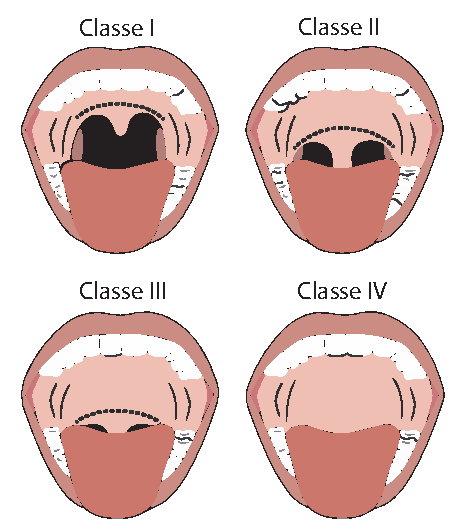
\includegraphics[width=0.6\textwidth]{Figure/mallampatpdf.pdf}
    \caption{Classificazione di Mallampati, adattata da \cite{Vargo2012}.}
    \label{fig:mallampati}
\end{figure}

\newpage

\section{Ambiente ed equipaggiamento}

Prima di procedere con la sedazione è indispensabile valutare l'idoneità dell'ambiente e del materiale, necessario per il monitoraggio del paziente o in caso di complicanze. \`E, quindi, importante, da un lato, che l'operatore abbia spazio a sufficienza per muoversi e raggiungere facilmente la testa del paziente in caso di necessità, dall'altro, che abbia verificato la presenza ed il funzionamento di tutta la strumentazione necessaria, oltre a conoscerne la precisa collocazione.

L'equipaggiamento da avere sempre a disposizione e da controllare prima di ogni sedazione può essere raggruppato in categorie, facilmente memorizzabili grazie all'acronimo inglese \texttt{SOAPME}, descritto nella tabella \ref{tab:soapme}.

\bgroup
\def\arraystretch{1.5}
\begin{table}[!h]
    \centering
    \begin{tabular}{p{0.05\textwidth} p{0.3\textwidth} p{0.6\textwidth}}
       
       \texttt{S} & Aspirazione (\emph{Suction}) & Sondini da aspirazione di dimensione adeguata ed un aspiratore funzionante \\ \hline
      \texttt{O} & Ossigeno & Erogatore di ossigeno a muro collegato preferibilmente ad un pallone va e vieni con una maschera di dimensione adeguata. Inoltre, è raccomandata la presenza di una bombola con una disponibilità di ossigeno sufficiente a garantire, in caso di complicanze, il trasporto del paziente nella struttura di emergenza o rianimazione \\ \hline
       \texttt{A} & Vie aeree (\emph{Airway}) & Equipaggiamento per la gestione delle vie aeree: cannule di Mayo, cannule nasofaringee, maschere laringee, set di intubazione (di dimensioni appropriate all'anatomia del paziente)\\ \hline
       \texttt{P} & Farmaci (\emph{Pharmacy)} & Tutti i farmaci fondamentali al supporto vitale del paziente in situazioni di emergenza, quali ad esempio adrenalina, amiodarone, atropina, beclometasone, salbutamolo, succinilcolina e flumazenil (antagonista del recettore GABA\ped{A})\\ \hline
       \texttt{M} & Monitoraggio & Strumenti indispendabili al monitoraggio del paziente, quali saturimetro (cons egnale acustico), capnografo, stetofonendoscopio e sfigmomanometro, monitor ECG\\ \hline
       \texttt{E} & Equipaggiamento & Disponibilità di un carrello o zaino di emergenza e di un defibrillatore\\
    \end{tabular}
    \caption{\texttt{SOAPME}: check list del materiale, adattata da \cite{Daud2014, Guidelines2019}}
    \label{tab:soapme}
\end{table}
\egroup

Oltre a ciò, è imprescindibile la presenza di almeno due professionisti sanitari durante la procedura, solitamente un medico ed un infermiere. Mentre il primo sceglie i sedativi da utilizzare ed esegue la procedura, il secondo ha il compito di controllare i parametri vitali ed i segni clinici del paziente, oltre a somministrare i farmaci \cite{Krauss2006, Simeupsedazione}. 

\section{Monitoraggio del paziente}